\documentclass[tikz, margin=3mm]{standalone}
\usepackage{tikz}
\usepackage{amsmath}
\usetikzlibrary{shapes.geometric, arrows, positioning}
\tikzstyle{arrow} = [thick,->,>=stealth]

% flow chart of simulation (zoomed out view)
% uses relative positioning

% Terminal
\tikzstyle{terminal} = [rectangle, rounded corners, minimum width=3cm, minimum height=1cm,text centered, text width=3cm, draw=black]

% Process
\tikzstyle{process} = [rectangle, minimum width=3cm, minimum height=1cm, text centered,text width=4cm, draw=black]

% Decision
\tikzstyle{decision} = [diamond, aspect=1.8, minimum width=2cm, minimum height=1cm, text centered, text width=2cm, draw=black]

% Subprocess
\newcommand\ppbb{path picture bounding box}
\tikzset{
	subprocess/.style = {rectangle, draw=black, 
		minimum width=4.3cm, minimum height=1cm, inner xsep=3mm,
		text width =\pgfkeysvalueof{/pgf/minimum width}-2*\pgfkeysvalueof{/pgf/inner xsep},
		align=flush center,
		path picture={\draw 
			([xshift =2mm] \ppbb.north west) -- ([xshift= 2mm] \ppbb.south west)
			([xshift=-2mm] \ppbb.north east) -- ([xshift=-2mm] \ppbb.south east);
		},% end of path picture
	}
}

\begin{document}
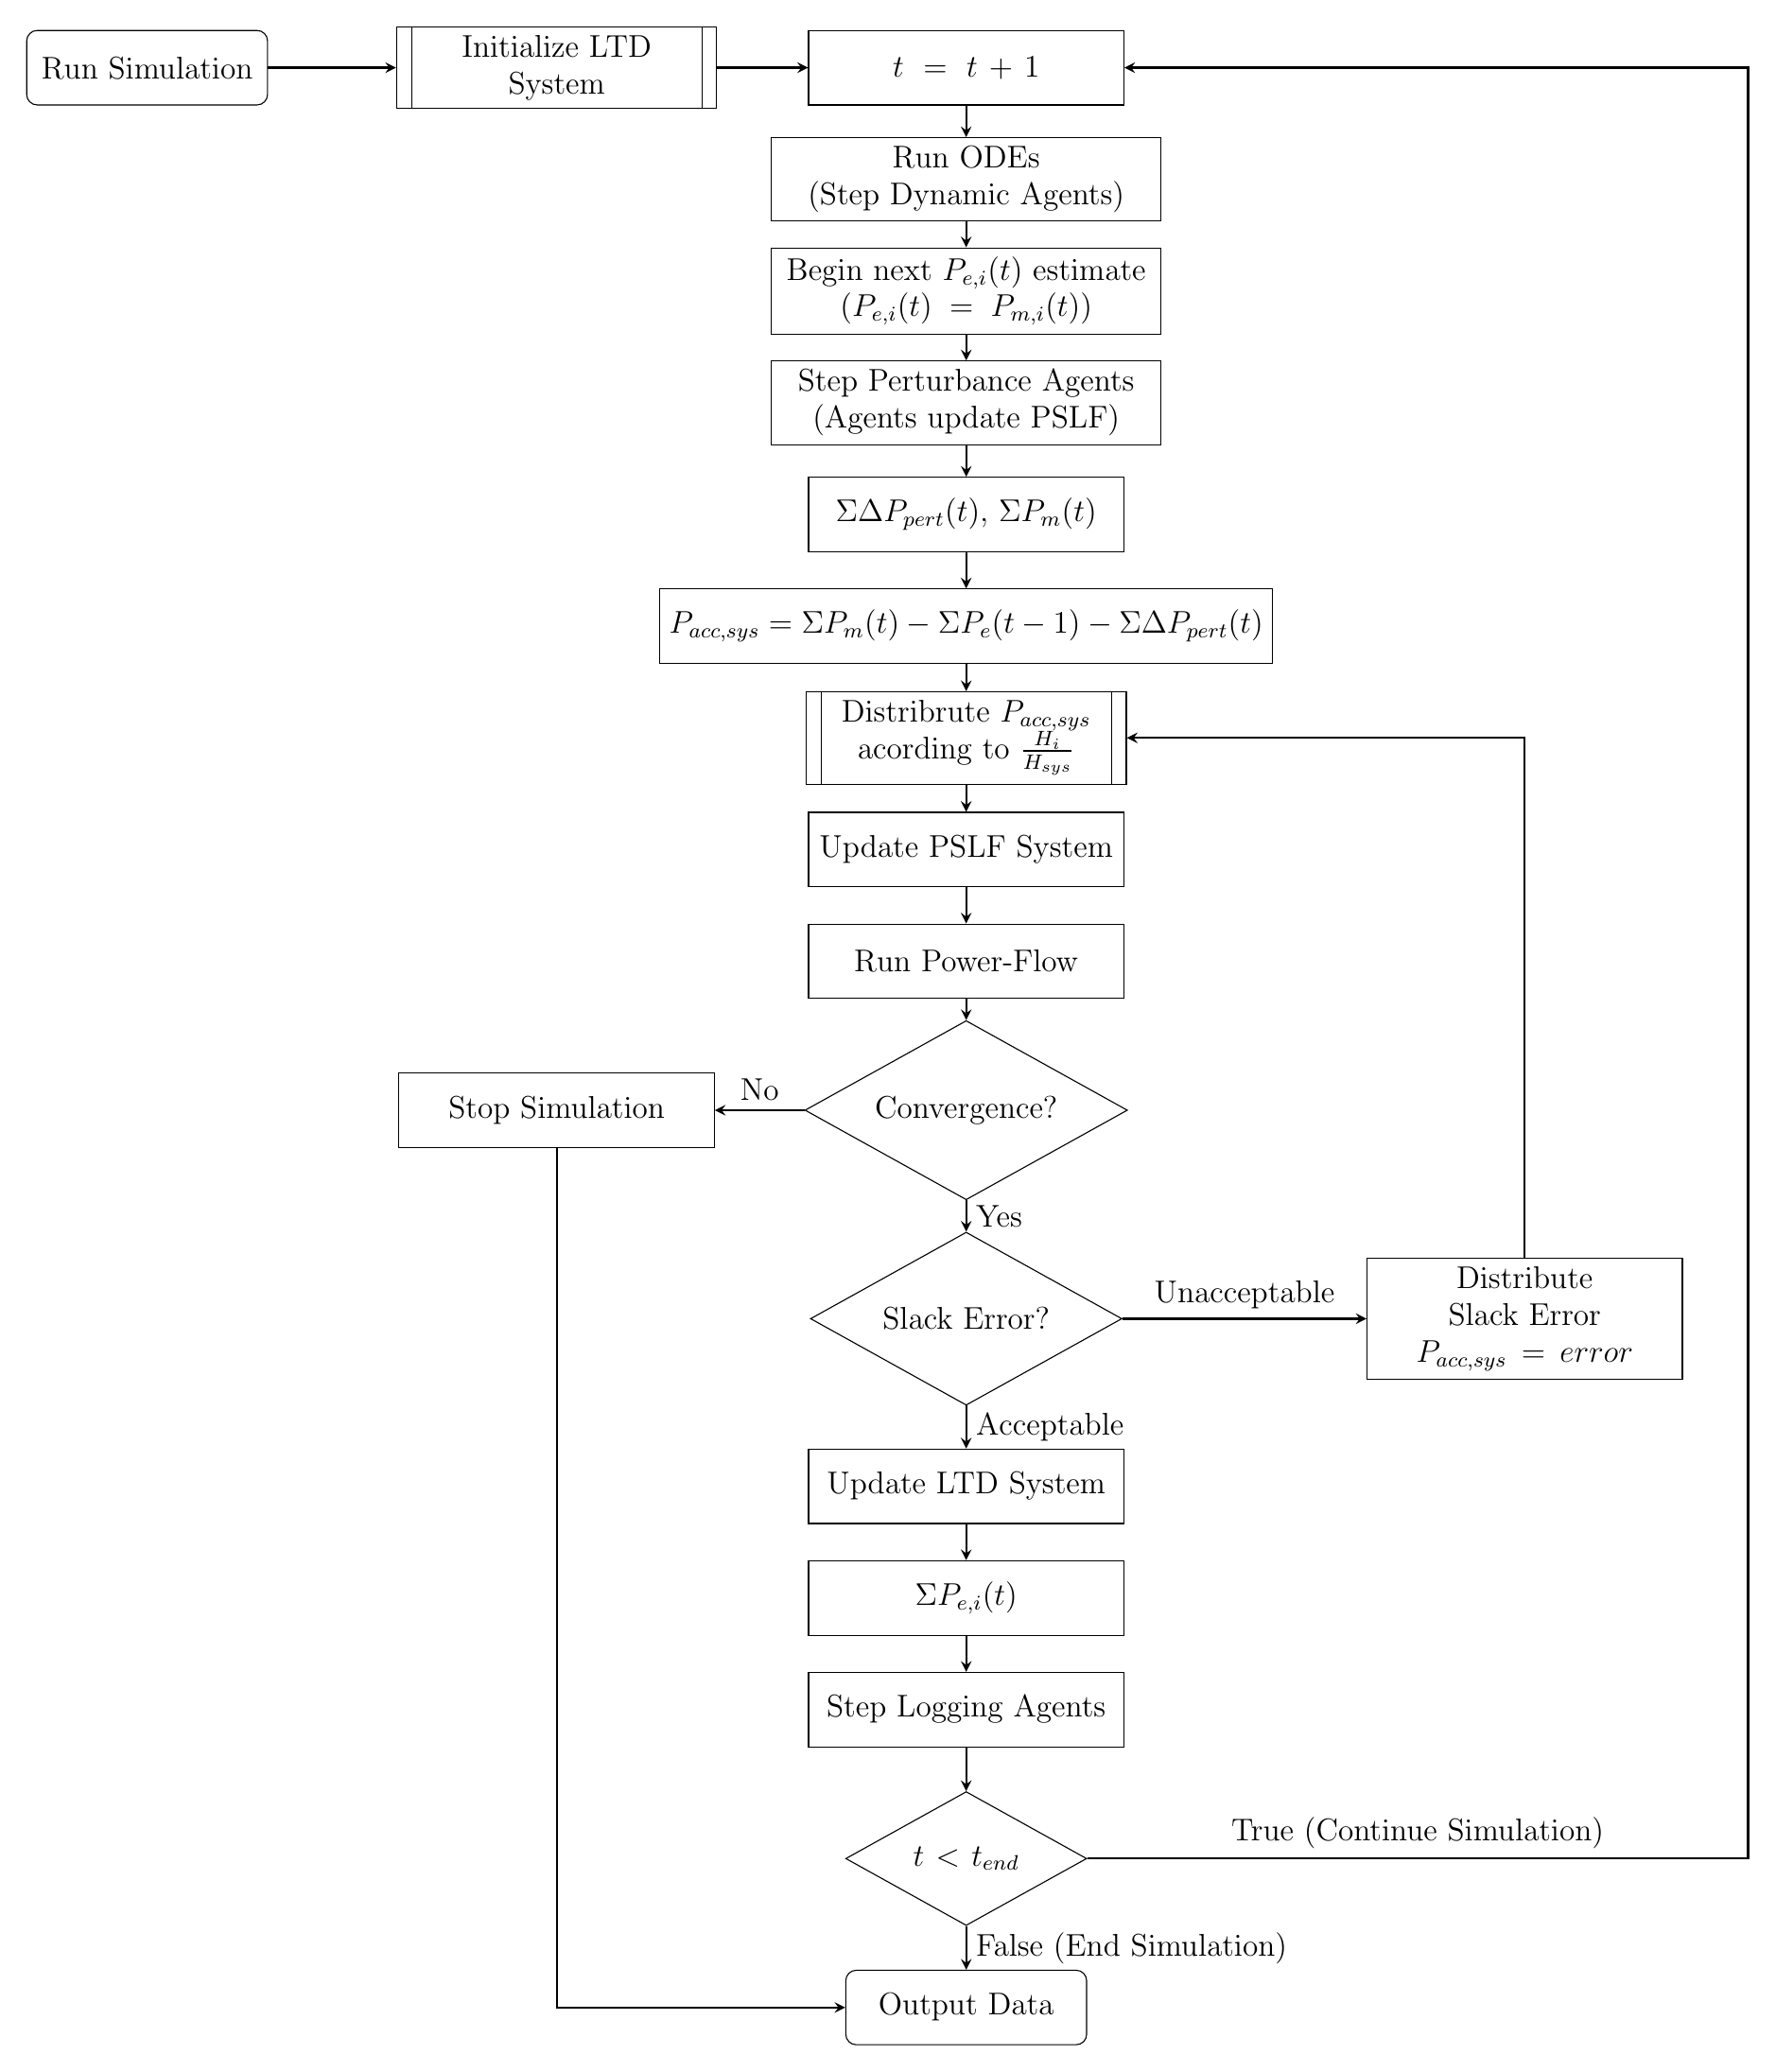
\begin{tikzpicture}[node distance=1.5cm, font=\large] 
% Placement of nodes
\node (start) [terminal] {Run Simulation};
\node (init) [subprocess, right of=start,xshift=4cm] {Initialize LTD System};
\node (tStep) [process, right of=init,xshift=4cm] {$t = t+1$};
\node (dyStep) [process, below of=tStep,text width=5cm] {Run ODEs \\ (Step Dynamic Agents)};
\node (PeEst) [process, below of=dyStep,text width=5cm] {Begin next $P_{e,i}(t)$ estimate \\ ($P_{e,i}(t) = P_{m,i}(t)$)};
\node (stepPert) [process, below of=PeEst, text width=5cm] {Step Perturbance Agents \\ (Agents update PSLF)};
\node (sumPertPm) [process, below of=stepPert, text width=4cm] {$\Sigma\Delta P_{pert}(t)$, $\Sigma P_{m}(t)$};
\node (calcPacc)[process, below of=sumPertPm,  text width=8cm] {$P_{acc, sys} = \Sigma P_m(t)-\Sigma P_e(t-1)- \Sigma \Delta P_{pert}(t)$};
\node (distPe) [subprocess, below of=calcPacc] {Distribrute $P_{acc, sys}$ \\acording to $\frac{H_i}{H_{sys}}$};
\node (updatePSLF) [process, below of=distPe] {Update PSLF System};
\node (runPF) [process, below of=updatePSLF,text width=4cm] {Run Power-Flow};

%Convergence nodes
\node (pfConv) [decision, below of=runPF, yshift=-.5cm, text width=3cm] {Convergence?};
\node (pfFail) [process, left of=pfConv, xshift=-4cm] {Stop Simulation};
%Slack error nodes
\node (slackErr) [decision, below of=pfConv, yshift=-1.3cm, text width=3cm] {Slack Error?};
\node (slackTol) [process, right of=slackErr, xshift=6cm] {Distribute Slack Error \\ $P_{acc, sys} = error$};

\node (updateLTD) [process, below of=slackErr,yshift=-0.75cm] {Update LTD System};
\node (sumPe) [process,below of=updateLTD] {$\Sigma P_{e,i}(t)$};
\node (log) [process, below of=sumPe, text width = 4cm] {Step Logging Agents};
\node (loop) [decision, below of=log, yshift=-.5cm] {$t<t_{end}$};
\node (dataOut) [terminal, below of=loop, yshift=-.5cm] {Output Data};

% Placement of edges
\draw [arrow] (start) -- (init);
\draw [arrow] (init) -- (tStep);
\draw [arrow] (tStep) -- (dyStep);
\draw [arrow] (dyStep) -- (PeEst);
\draw [arrow] (PeEst) -- (stepPert);
\draw [arrow] (stepPert) -- (sumPertPm);
\draw [arrow] (sumPertPm) -- (calcPacc);
\draw [arrow] (calcPacc) -- (distPe);
\draw [arrow] (distPe) -- (updatePSLF);
\draw [arrow] (updatePSLF) -- (runPF);
\draw [arrow] (runPF) -- (pfConv);

% pf convergence bad
\draw [arrow] (pfConv) --  node[anchor=south] {No} (pfFail);
\draw [arrow] (pfFail) |-  (dataOut);
% pf convergence ok
\draw [arrow] (pfConv) --  node[anchor=west] {Yes} (slackErr);

% slack tolerance bad
\draw [arrow] (slackErr) --  node[anchor=south] {Unacceptable} (slackTol);
\draw [arrow] (slackTol) |- (distPe);
% slack tolerance ok
\draw [arrow] (slackErr) --  node[anchor=west] {Acceptable} (updateLTD);

\draw [arrow] (updateLTD) --(sumPe);
\draw [arrow] (sumPe) --(log);
\draw [arrow] (log) --(loop);

%loop again
\draw [arrow] (loop) -- node[anchor=south, midway] {True (Continue Simulation)} +(10.5,0) |- (tStep);
% end simulation
\draw [arrow] (loop) -- node[anchor=west] {False (End Simulation)} (dataOut);

\end{tikzpicture}
\end{document}
